\documentclass[12pt,a4paper]{article}
\usepackage{amssymb}
\usepackage{fullpage}
\usepackage{graphicx}
\author{Parker Whaley}
\title{lab \#1}
\begin{document}

\maketitle

\section{Abstract}
This experament was conducted to determine the speed of light for various wevelengths of light in glass.  We did this by using a triangular prisim made of glass.

\section{Tabulation of data}
\subsection{Triangle Apex Angle}
These are the mesured angles of reflection, there were two vewing windows one next to the bar code and another, they are denoted accordingly.  The uncertenty in our mesures of the angles was $\delta\theta=1'$\\
\begin{tabular}{| l | l | l |}
\hline
  & $\theta_{bar}$ & $\theta_{\circ}$\\
\hline
$\theta_1$ & $\theta_a= 297^\circ 10'$ & $\theta_c =117^\circ 10'$\\
\hline
$\theta_2$ & $\theta_b= 57^\circ 14'$ & $\theta_d= 237^\circ 14'$\\
\hline

\end{tabular}
\\

\begin{tabular}{c c}

$\theta_a$ & $\theta_b$\\
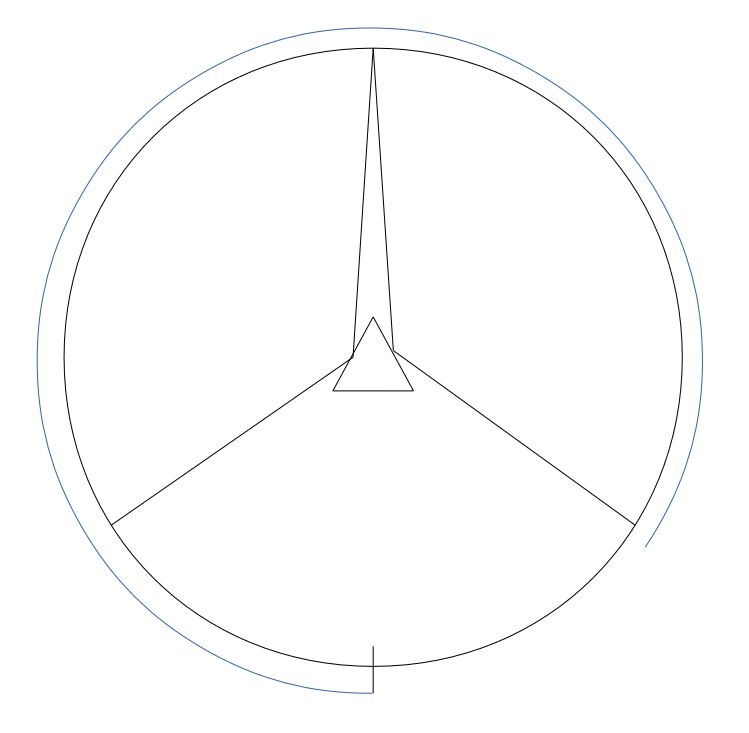
\includegraphics[scale=.15]{a2} & 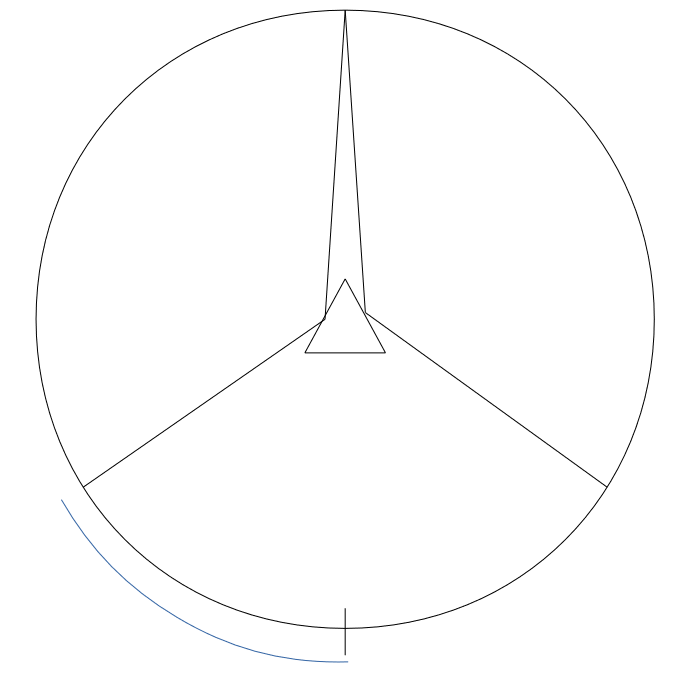
\includegraphics[scale=.15]{a1}\\
$\theta_c$ & $\theta_d$\\
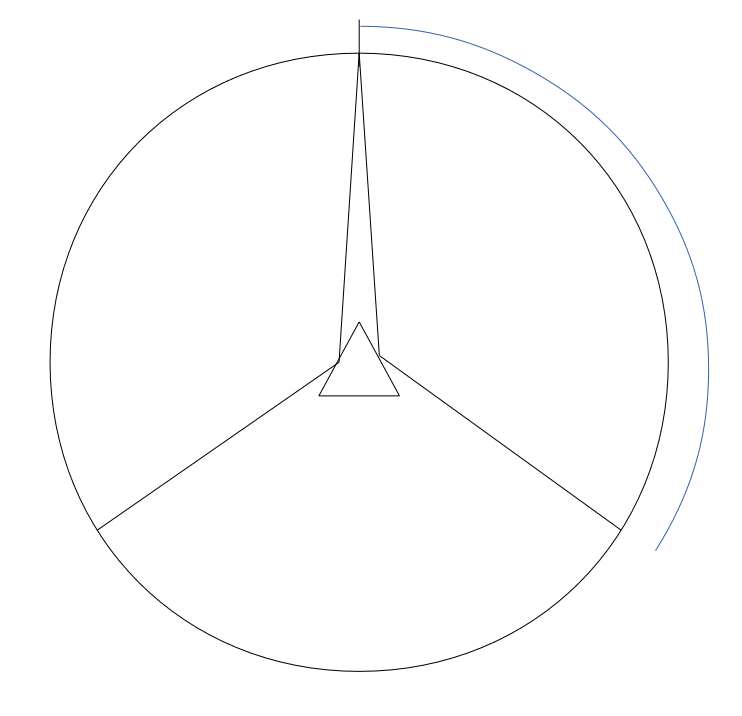
\includegraphics[scale=.15]{a3} & 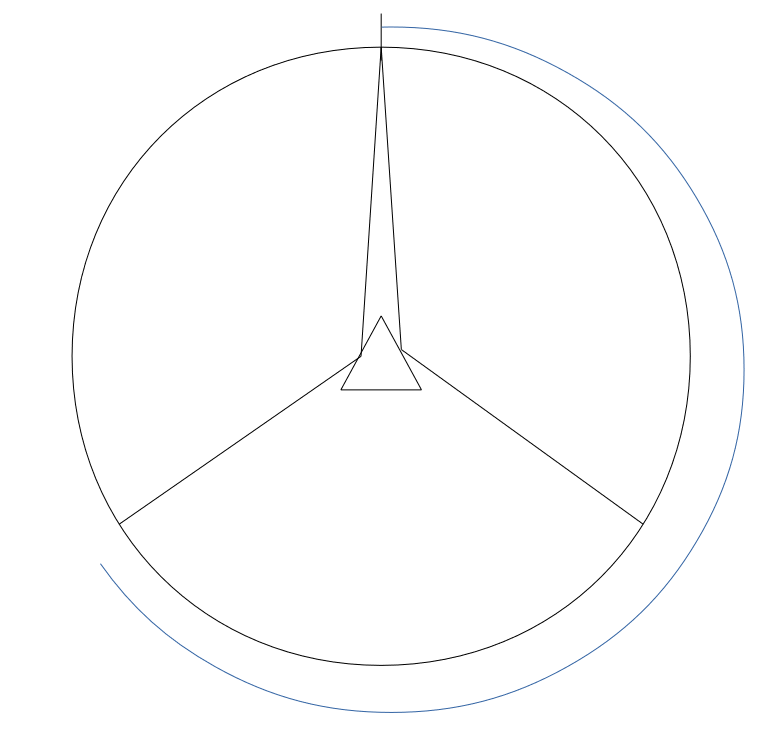
\includegraphics[scale=.15]{a4}

\end{tabular}
\subsection{Divergence in Angle}
Here I have tabulated the minimum divergence of the light beeing transmitted thrught the prisim.  Eghther divergence from 0 in the case of $\phi_{bar}$ or divergence from 180 in the case of $\phi_\circ$.  Note that as before all angles carry the same uncertenty $\delta\phi=.5'$.  The last entry is the average of the two deviations $\phi_{ave}=\frac{\phi_{bar}+\phi_{\circ}-180}{2}$ and carrys a uncertenty of $\delta\phi_{ave}=2^{-3/2}$.

\begin{tabular}{| l | l | l | l |}
\hline
color & $\phi_{bar}$ & $\phi_\circ$ & $\phi_{ave}$\\
\hline
yellow & $38^\circ 39'$ & $218^\circ 39'$ & $38^\circ 39'$\\
\hline
blue & $39^\circ 15'$ & $219^\circ 15'$ & $39^\circ 15'$\\
\hline
green & $39^\circ 1'$ & $219^\circ 1'$ & $39^\circ 1'$\\
\hline
red & $38^\circ 25'$ & $218^\circ 25'$ & $38^\circ 25'$\\
\hline
purple & $39^\circ 25'$ & $219^\circ 25'$ & $39^\circ 25'$\\
\hline


\end{tabular}
\subsection{Images}
This is the image seen thrugh the scope of the diviation between the diferent colors in the helium spectra:\\
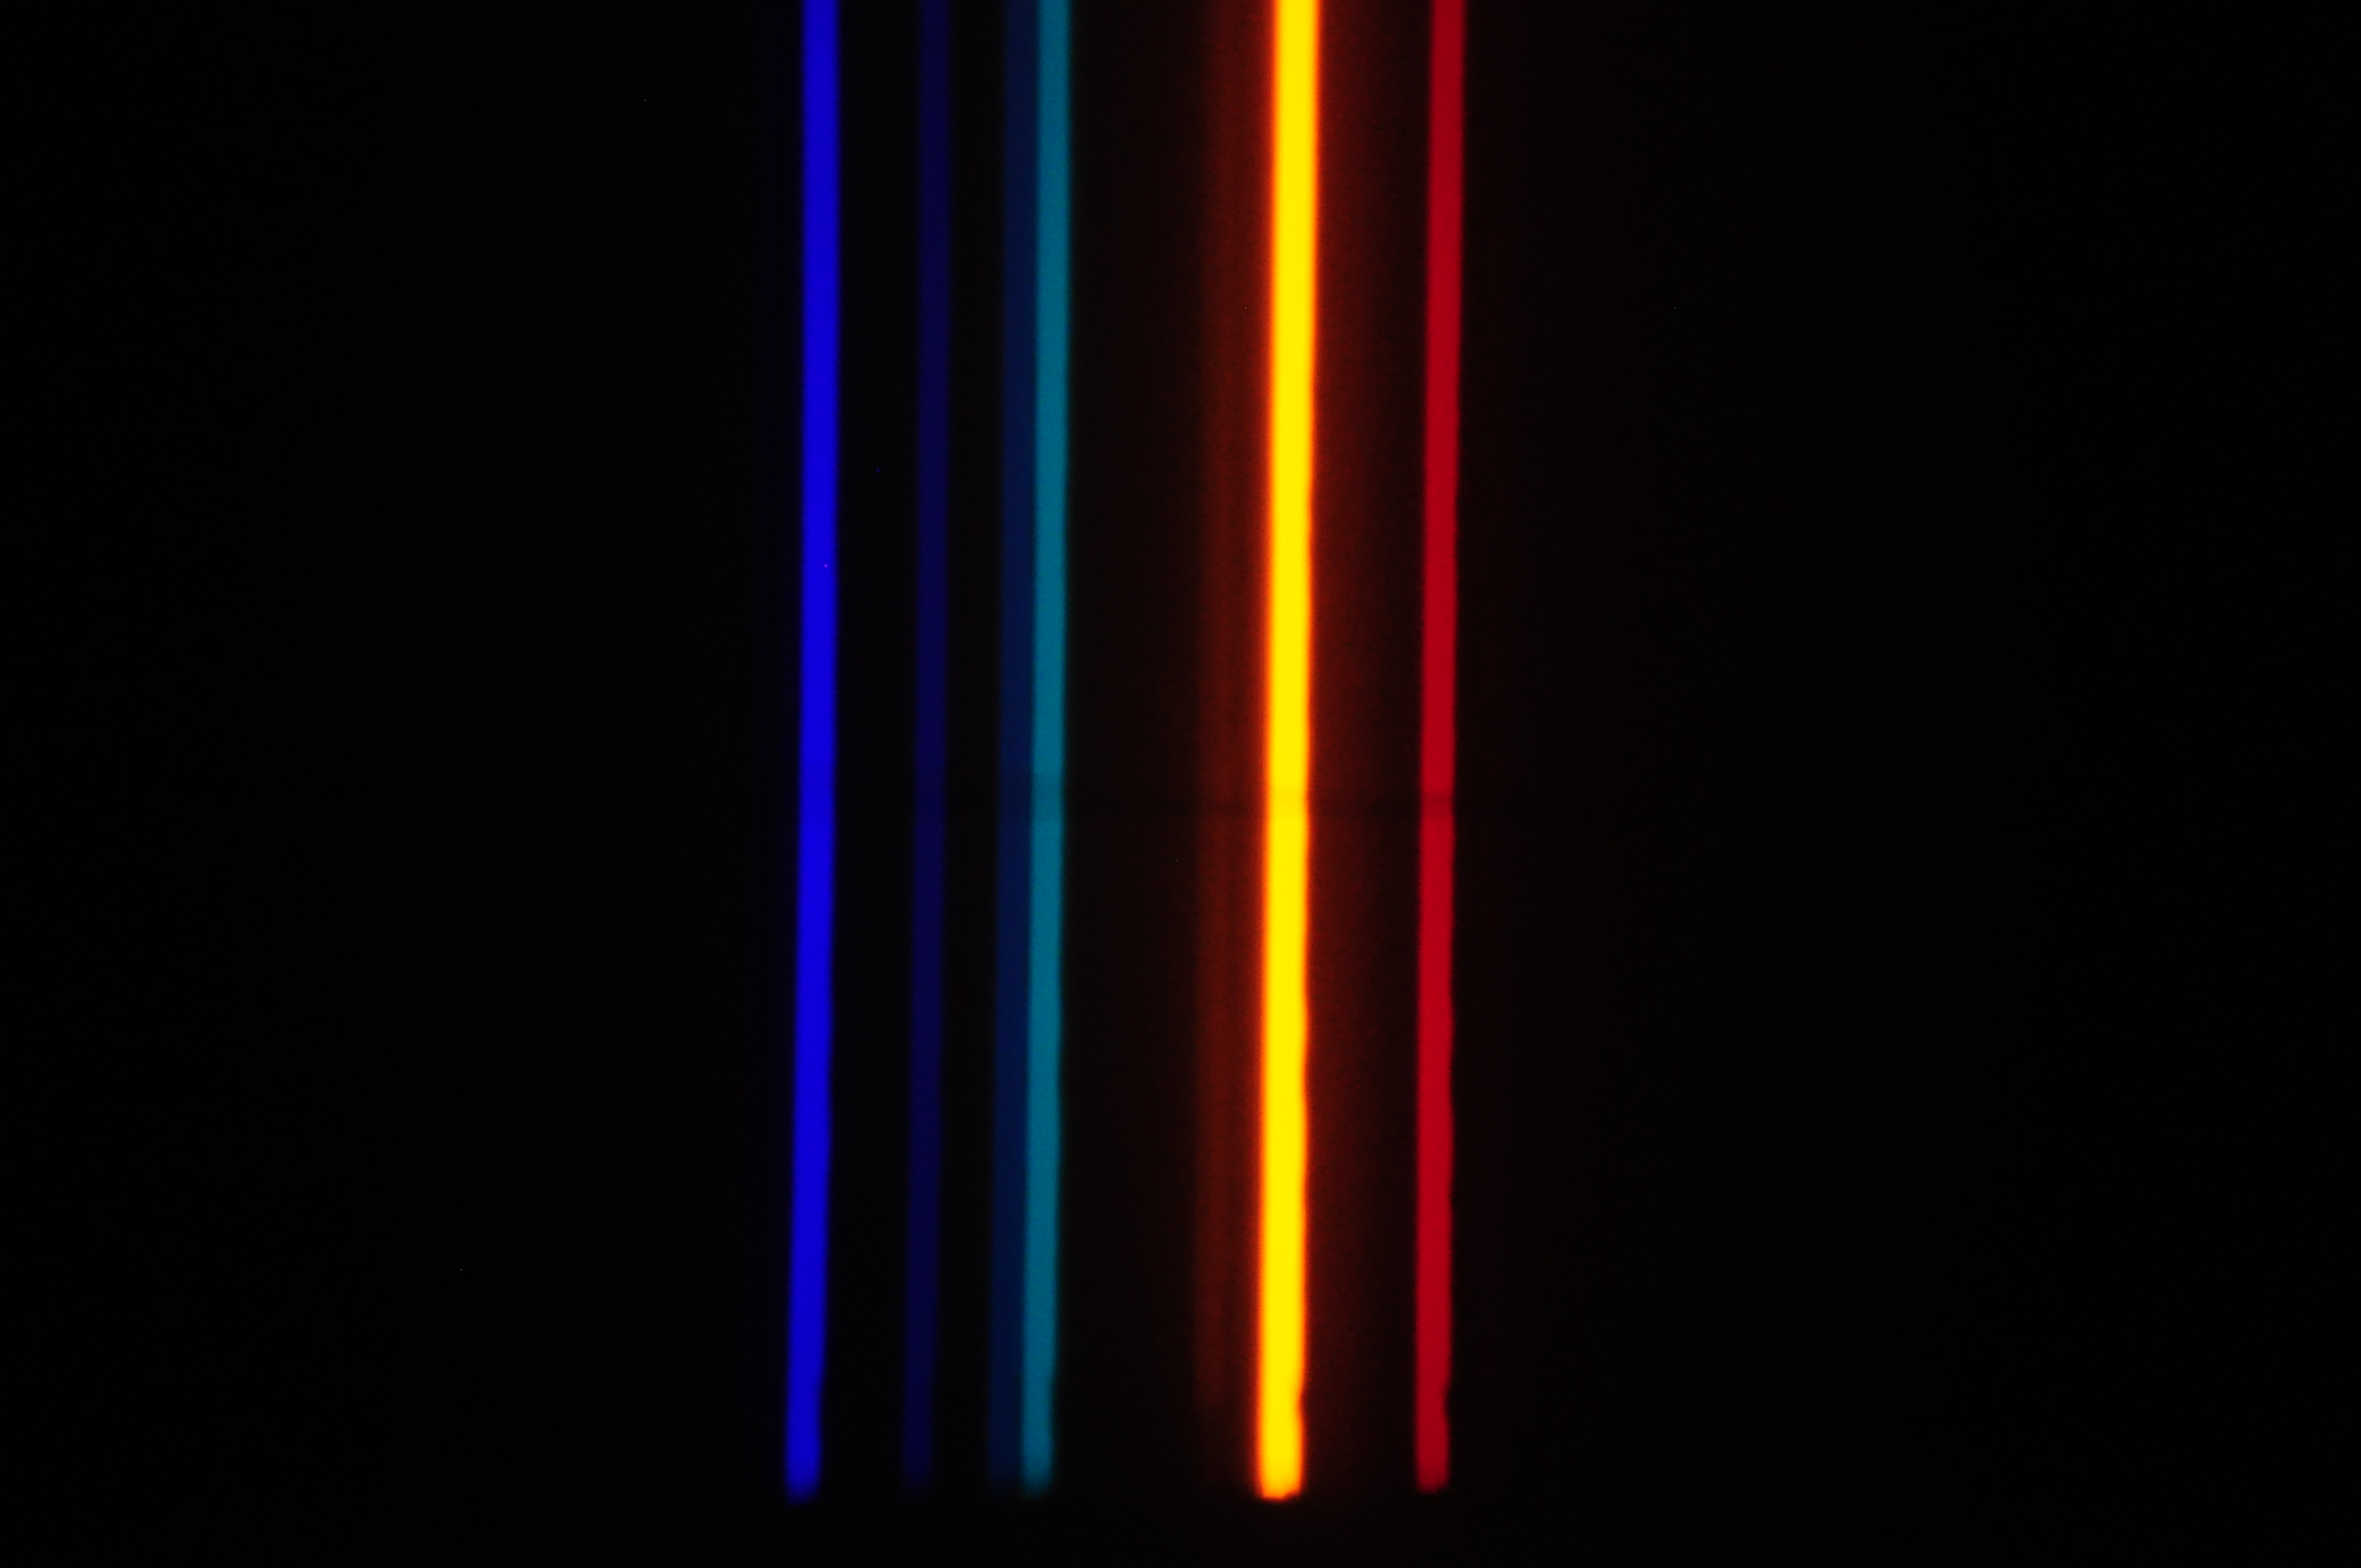
\includegraphics[scale=.3]{hspec}\\
This is the spectral intencity comming directly off the helium tube:\\
PUT THIS IN!!!!!!!!!!


\section{Analasis of Results}
First we must determine the angle of the apex of the prisim call this angle $\alpha$, the angle between the two faces we pass the light thrugh.  We are given that this angle must be half the angle between the two reflected beams.  We can calculate this angle two ways, $\alpha=\frac{\theta_d-\theta_c}{2}$ and $\alpha=\frac{(360-\theta_a)+\theta_b}{2}$.  Lets average these two methods and use that average angle as our $\alpha$:
\[\alpha=\frac{\theta_d-\theta_c+360-\theta_a+\theta_b}{4}\]
We can also get the uncertenty in this angle (note all $\theta$s have the same uncertenty:
\[\delta\alpha^2=\Sigma(\frac{\partial\alpha}{\partial\theta_i}*\delta\theta_i)^2=(1/16*4)\delta\theta^2=(.5')^2\]
Also plugging in the above values for the various $\theta$s we arrive at:
\[\alpha=60^\circ 2'\pm .5'\]
I am given the equation for the index of refraction as:
\[n=\frac{\sin((\phi+\alpha)/2)}{\sin(\alpha/2)}\]
We can do normal uncertenty analasis procedure as done with $\alpha$ above to find the uncertenty in n:
\[\]














\end{document}